\documentclass{article}
\usepackage{PRIMEarxiv}
\usepackage[utf8]{inputenc}
\usepackage[T1]{fontenc}
\usepackage{amsmath,amsfonts,booktabs,graphicx,microtype,nicefrac,fancyhdr}
\usepackage[hidelinks]{hyperref}
\pagestyle{fancy}
\fancyhead[LO]{Receiver-Aware Communication for Search-and-Rescue}
\rhead{}

\newcommand{\MV}{\operatorname{MV}}
\newcommand{\VoC}{\operatorname{VoC}}
\newcommand{\Agree}{\operatorname{Agree}}
\newcommand{\E}{\mathbb{E}}
\newcommand{\indicator}{\mathbf{1}}

\title{Receiver-Aware Value of Communication for Cooperative Multi-Agent Search-and-Rescue}
\author{Chitiveli Hemcharan Varma (24110095), Guransh Kaur Saran (24110127),\\
Kowel P Laloo (24110168), and Omm Arindam (24110229)\\
Indian Institute of Technology Gandhinagar\\
Group 27}
\date{November 22, 2026}

\begin{document}
\maketitle
\thispagestyle{empty}

\begin{abstract}
A Scout may know where a victim is while the nearby Medic does not. The value of sending that location depends on who can act on it, who already knows it, and how much time is available for the consequences to unfold. We study this decision in a partially observed three-agent search-and-rescue simulator. A sender uses a receiver-conditioned particle model and paired send/no-send rollouts to score structured reports. A ten-seed evaluation contains 120 episodes and 100 separate oracle contexts. Five-step valuation improves agreement with a 15-step oracle by 46.3 percentage points on 41 delayed-value contexts. Raising the software cost from 0 to 0.5 lowers the positive-value send rate by 89.8\%. Only 3 of 89 eligible contexts meet the prespecified receiver-differentiation threshold. Receiver-aware valuation reduces traffic by 85.9\% relative to the always-send baseline under the discounted-return equivalence criterion, but the paired return interval at an assigned two-message budget includes zero. At zero cost the receiver-aware policy also rescues fewer victims than the always-send baseline. The results support downstream valuation and cost-sensitive sending in this setting, with limited evidence for a receiver-aware advantage at equal traffic.
\end{abstract}

\keywords{search-and-rescue \and decentralized decision-making \and value of communication \and paired simulation}

\section{Introduction}

A Scout finds a victim in a building. The Medic can stabilize the victim, while the Carrier can move the victim only after stabilization. A location report to the Medic may therefore help immediately, while the same report to the Carrier may do little at that point. Even the Medic may gain nothing if the victim is already in view. The report is identical in all three cases. Its value changes with the recipient's job, current information, and ability to reach the victim.

A team with limited visibility needs to exchange some of these reports. Sharing every available report takes communication opportunities away from other information. A stale hazard report can also change a route in an unhelpful direction. A system that charges a cost per send needs to decide when to transmit, which teammate to address, and which existing information item to share. Physical radio effects are outside our setting. The cost is a software-level quantity in the same units as task reward.

The time horizon matters as well. A Medic may take several steps to reach a newly located victim. On the step of delivery both the send and no-send teams may earn the same reward, even if their routes have already diverged. A longer rollout can reveal some of those differences. It also gives prediction errors more time to accumulate, especially when hazards move or change activity.

We ask whether estimating a report's value for a particular receiver improves selective communication relative to a receiver-independent comparator and a one-step valuation. The sender first shortlists plausible report--recipient pairs using local evidence. It then simulates each shortlisted pair twice, delivering the message in one branch and withholding it in the other. A separate evaluator uses complete simulator context to estimate the effect of that same intervention. This gives two tests with different endpoints: whether the selected action matches the evaluator, and whether an online policy improves full-episode outcomes under controlled communication.

The experiment isolates these endpoints with fixed task policies, matched scenario seeds, a prospective message budget, and an explicit cost sweep. We report both discounted return and the number of victims evacuated. These outcomes diverge in our runs because discounting values early rewards much more heavily than late rescues.

\section{Background and problem formulation}

Value of information measures the expected utility gained from having information \cite{howard1966}. Communication in cooperative multi-agent systems adds a choice about who acquires the information and when \cite{xuan2001}. Targeted learned communication and counterfactual message valuation address related routing and credit-assignment problems \cite{das2019,gao2025}. Our experiment uses structured reports and fixed policies to measure those effects without training a communication network.

We model the task as a cooperative decentralized partially observable Markov decision process \cite{oliehoek2016}. The simulator holds the global state $S_t$, including agent positions, victim and hazard states, carrier assignments, hazard disable timers, and time. Each agent receives its local observation and retains local memory. The notation $h_i^t$ denotes the sender's accessible history, represented in the implementation by the current local observation, remembered facts and teammate tracks, and prior sends. The ideal recipient belief $P(S_t\mid h_j^t)$ conditions on recipient $j$'s private history. The sender instead constructs an approximate model distribution $\widehat b_{j,t}$ from its own evidence, the recipient's role $K_j$, and its record $\ell_{ij,t}$ of reports it sent to $j$.

The Scout scans cells for victims and hazards. The Medic stabilizes located victims and can temporarily disable active hazards. The Carrier picks up stabilized victims and delivers them to a fixed evacuation cell. A victim becomes rescued on delivery. The team receives the event reward
\begin{equation}
 r_t=10n_t^{\mathrm{resc}}+n_t^{\mathrm{loc}}+2n_t^{\mathrm{stab}}-0.05N ,
 \label{eq:reward}
\end{equation}
where the three $n$ terms count rescues, newly located victims, and stabilizations on step $t$, and $N=3$ is the number of task-action slots charged per step, including waits. Let $T$ be the actual episode length. The episode ends at the step cap or after the last victim is rescued. The returns used in the paper are
\begin{equation}
 J_t^H=\sum_{u=t}^{\min(t+H,T)-1}\gamma^{u-t}r_u,\qquad
 J_0=\sum_{u=0}^{T-1}\gamma^u r_u .
 \label{eq:return}
\end{equation}
The clock begins at zero. The horizon $H$ counts transitions beginning with the delivery step, and each branch stops at its own terminal time. Undiscounted rescue count sums $n_t^{\mathrm{resc}}$ over the full episode.

Before each task step the Scout may send one directed report or stay silent. Candidate reports $\mathcal M_i(t)$ come from remembered victim and hazard facts and the Scout's current task intention. Decisions use the pre-delivery observation. Delivery precedes the task actions, which precede the simulator transition. The other agents do not send in the primary experiment. For an information context $\mathcal I$ and fixed continuation policies, define
\begin{equation}
 \MV^H_{i\to j}(m,t\mid\mathcal I)
 =\E[J_{t,\mathrm{send}}^H-J_{t,\mathrm{no}}^H\mid\mathcal I],
 \qquad
 \VoC^H_{i\to j}=\MV^H_{i\to j}-\lambda c_0 .
 \label{eq:voc}
\end{equation}
Here $m$ is the report, $i$ is the sender, $j$ is the recipient, and $\lambda c_0$ is the cost of that single report. Equation~\eqref{eq:reward} excludes communication cost. We subtract it once when deciding whether to transmit.

\section{Methodology}

\subsection{Receiver model and candidate filtering}

The particle filter maintains a separate cached ensemble for each sender and recipient. At a later decision it propagates surviving particles under the fixed task policies and weights the predictions by agreement with local evidence. Resampling is proportional to positive heuristic weights $w_p$, so a prediction is drawn with probability $w_p/\sum_q w_q$. The code downweights disagreement with observed agent positions and current fact statuses. With an available predicted ensemble, 48 of the 64 output particles descend from weighted draws and 16 are refreshed from the observation-conditioned simulator prior. Without a surviving prediction, all particles are freshly constructed. Reconstructed worlds incorporate current sender facts and visible positions, sample locations for unobserved entities, and initialize recipient memory using the sender's delivery record. Recipient task observations come from the reconstructed world and its modeled memory. The procedure uses the structure of sequential Monte Carlo \cite{gordon1993}; its weights and reconstruction are approximations to the recipient's information state.

Let $\kappa=\max(0,t-t_{\mathrm{obs}})$ be report age and let $\nu_{mj}$ be the novelty score derived from the delivery record. The shortlist score is
\begin{equation}
 s_{mj}=u(m,K_j)\,\nu_{mj}\,
       [(1-p_{\mathrm{move}})(1-p_{\mathrm{toggle}})]^\kappa
       \left(\frac{1}{2}+\frac{\rho_{mj}}{2}\right).
 \label{eq:shortlist}
\end{equation}
Here $u$ is a fixed role-compatibility lookup, and $\rho_{mj}=1/(1+d_{mj})$ uses the Manhattan distance from the last tracked recipient position to the report location. When no track is available the proximity factor uses $\rho_{mj}=1$. The freshness factor is a ranking feature. An unchanged fact already delivered with an equal or newer timestamp receives zero novelty. The algorithm scores at most eight pairs with the rollout estimator after ranking. Shortlisting can omit the best pair, so we measure its coverage against all candidates offline.

\subsection{Paired estimation and selection}

For each candidate, a rollout pair draws a particle uniformly from the reconstructed ensemble, clones the resulting initialized context, and uses the same dynamics seed for the two branches. In the send branch the candidate arrives at time $t$. In the no-send branch it is withheld. Both branches run the same deterministic task policies with no further messages over the remainder of the rollout. With $B$ paired draws,
\begin{equation}
 D_k=J_{t,k,\mathrm{send}}^H-J_{t,k,\mathrm{no}}^H,\qquad
 \widehat{\MV}^{\,H}_{i\to j}=\frac{1}{B}\sum_{k=1}^{B}D_k,\qquad
 \widehat{\VoC}^{\,H}_{i\to j}=\widehat{\MV}^{\,H}_{i\to j}-\lambda c_0 .
 \label{eq:estimator}
\end{equation}
Matching the stochastic inputs can reduce the variance of $D_k$ through positive covariance between branch returns \cite{glasserman1992}. The difference still targets the return under the chosen initialization and continuation model. Common randomness cannot remove errors caused by estimated beliefs, horizon truncation, or model mismatch. We use the first pair in shortlist order among equal maximizers and transmit only if its score is strictly positive in unrestricted valuation.

\begin{figure}[t]
\centering
\begin{minipage}{0.95\linewidth}
\small
\begin{tabular}{@{}r p{0.86\linewidth}@{}}
\toprule
Step & Receiver-aware decision at time $t$\\
\midrule
1 & Read local observations, remembered facts, tracks and prior deliveries. Form $\mathcal M_i(t)$.\\
2 & Rank candidate pairs by Eq.~\eqref{eq:shortlist}; keep up to $N_{\mathrm{short}}$.\\
3 & For each shortlisted $(m,j)$, update or retrieve $\widehat b_{j,t}$. Draw $B$ contexts and run matched branches for $H$ steps.\\
4 & Subtract $\lambda c_0$ and choose the largest estimated value. In unrestricted operation send only if this maximum is positive.\\
5 & Deliver any selected report, let all agents act on their own updated observations, and advance the environment.\\
\bottomrule
\end{tabular}
\end{minipage}
\caption{Decision procedure. The actual simulator context enters only the separate offline oracle, never the online scoring interface.}
\label{fig:algorithm}
\end{figure}

The agnostic valuation applies a message-only shortlist. It strips actual teammate tracks and delivery summaries from the scoring input, then averages the values for a fixed synthetic Carrier and Medic with equal weight and 16 pairs per role. The real recipient is selected by a fixed seeded rule independent of its estimated value. Thus the same local message has one score under this comparator, regardless of the actual recipient. Aware valuation can differ by role, belief, and recipient; it also uses a different shortlist. The budget experiment compares complete policies incorporating these design choices. Figure~\ref{fig:algorithm} summarizes the aware procedure.

\subsection{Offline reference and diagnostic metrics}

The oracle clones the true simulator context, including the agents' modeled memories at the decision point, and estimates $D_k$ with independently seeded batches of 128 pairs. It ranks all admissible pairs against the no-send action of value zero. The main reference horizon is 15 steps. A separate one-step oracle estimate is used to classify delayed-value cases. The online methods use horizons 1 and 5. The exploratory horizon ablation separately tests longer online-estimator horizons in an offline study. Primary oracle decisions are never used to select a message during episode execution.

For context $q$ write $V_q^\star(a)$ for the finite Monte Carlo oracle value of communication action $a$, with $V_q^\star(\varnothing)=0$ and cost zero in the diagnostics. Pair regret is $\max_a V_q^\star(a)-V_q^\star(\widehat a_q)$. Receiver regret, evaluated only when a report is selected, holds that report fixed and subtracts the value of its chosen receiver from the best receiver value. The estimation error is the mean over contexts of the mean absolute error across the five-step shortlist, compared with the 15-step oracle. This gap includes horizon mismatch. Recall is the mean fraction of oracle pairs with value greater than $0.5$ that were shortlisted, restricted to contexts with at least one such pair. Usefulness is the fraction of selected sends with strictly positive oracle marginal value.

\section{Experimental setup}

\begin{table}[t]
\caption{Primary evaluation configuration. Targets and analysis denominators are specified in the text.}
\label{tab:config}
\centering
\begin{tabular}{@{}lp{0.60\linewidth}@{}}
\toprule
Parameter & Value and interpretation\\
\midrule
$N$, $L$ & Three roles (Scout, Carrier, Medic); $10\times 10$ grid\\
Victims, hazards, evacuation & Three victims; two hazards; delivery cell $(0,0)$\\
$p_{\mathrm{move}}$, $p_{\mathrm{toggle}}$ & $0.2$, $0.2$; hazard transition controls\\
$T_{\max}$, $\gamma$ & 100 transitions maximum; discount $0.8$\\
Task reward & $10$ rescue, $1$ locate, $2$ stabilize, $-0.05$ per agent-step\\
$N_p$, $N_{\mathrm{short}}$ & 64 model particles per ensemble; at most eight evaluated pairs or messages\\
$B$, $B_{\mathrm{oracle}}$ & 32 online pairs per score; 128 offline pairs per candidate and oracle horizon\\
$H_{\mathrm{myo}},H_{\mathrm{NM}},H_{\mathrm{eval}}$ & $1,5,15$ transitions, respectively\\
$\lambda$, $c_0$ & $0$ or $0.5$ for valued policies; unit cost $1$\\
Episode seeds and counts & 1000--1009; one episode per seed per condition, 120 total\\
Diagnostic contexts & 100 no-send contexts; ten scheduled steps per seed on separate layouts\\
Budget and equivalence & Two assigned messages; return margin $\pm 0.25$\\
\bottomrule
\end{tabular}
\end{table}

Table~\ref{tab:config} describes the primary run. We compare four baselines and six unrestricted valuation conditions: aware at each horizon and agnostic at horizon five, at each cost. Never suppresses all messages. Random sends a uniformly selected admissible report to a uniformly selected teammate on eligible steps. Full sends one heuristically ranked pair on each eligible step. Fixed-frequency sends the top-ranked pair every third step when a candidate is available. Full is thus an always-send single-slot baseline. The earlier proposal's share-all interpretation would have violated this capacity control.

In the two additional assigned-budget conditions, a sender must send at its first two eligible steps. The eligible set consists of located or stabilized victim reports and currently observed active hazards. A previously sent kind--location--status triple cannot spend another slot. Intention reports cannot spend the assigned budget. The rule and quota are common to both arms, and the state-dependent send times can differ after the trajectories diverge. All ten pairs in the recorded run used both slots. We pair episodes by seed, hold the task policies fixed, and keep the unrestricted and forced-budget episodes separate.

For diagnostic contexts the runner seeds a separate no-send trajectory with the episode seed plus 77,777, sampling evenly spaced steps across the cap. An H1-eligible context has a non-intention report; both receivers are evaluated for the first such report in candidate order. H1 asks whether at least $30\%$ of those contexts have an absolute oracle marginal-value gap greater than $0.5$ for that same report. For H2 the reduction against Full is $1-M_{\mathrm{aware}}/M_{\mathrm{Full}}$ using total sends at $\lambda=0$. Its target is $0.20$ at matched return, operationalized by the paired return interval lying inside $(-0.25,0.25)$. The assigned-budget half of H2 requires the paired Aware-minus-Agnostic return interval to exclude zero.

A context is delayed for H3 if at least one admissible pair has an absolute difference greater than $0.5$ between its 15-step and one-step oracle marginal values. For this subset $\mathcal D$ we compute
\begin{equation}
 \Agree(H,15)=\frac{1}{|\mathcal D|}
 \sum_{q\in\mathcal D}\indicator\{\widehat a_{q,H}=a^{\mathrm{oracle}}_{q,15}\}.
 \label{eq:agreement}
\end{equation}
An exact match requires the same recipient and report, or agreement on silence. H3 tests whether five steps improve this agreement by at least $0.10$ over one step. For H4, let $\bar r_\lambda$ be the mean across seeds of sends divided by eligible valuation opportunities in unrestricted aware five-step episodes. The target is a relative drop $1-\bar r_{0.5}/\bar r_0\ge 0.15$. A seed with zero sends and a positive opportunity count contributes a zero rate; a zero opportunity denominator is undefined. The relative drop requires a positive pooled baseline rate. In this run both costs have valid denominators on all ten seeds.

We use 95\% percentile bootstrap intervals from 10,000 seed resamples for the independent analysis. Each draw keeps a seed's paired conditions and diagnostic contexts together, recomputing the relevant fraction, paired difference, or ratio. The two versions of the experiment on the same seeds are reproducibility checks and contribute one observation per seed to a comparison. Individual contexts and Monte Carlo rollouts do not increase the number of independent episode replicates. Intervals describe uncertainty for the specified estimands; exploratory contrasts are reported separately without a family-wide discovery claim.

\section{Results}

\begin{tabular}{@{}lrrrr@{}}
\toprule
Policy & $\lambda$ & Mean $J$ [95\% CI] & Messages & Rescues \\
\midrule
Never & 0 & $-0.470\; [-0.735, -0.136]$ & 0 & 2 \\
Random & 0 & $-0.383\; [-0.709, -0.013]$ & 947 & 19 \\
Full & 0 & $-0.424\; [-0.725, -0.050]$ & 957 & 17 \\
Fixed-frequency & 0 & $-0.428\; [-0.727, -0.054]$ & 323 & 20 \\
Aware ($H=1$) & 0 & $-0.470\; [-0.735, -0.136]$ & 0 & 2 \\
Aware ($H=5$) & 0 & $-0.399\; [-0.716, -0.009]$ & 135 & 10 \\
Agnostic ($H=5$) & 0 & $-0.427\; [-0.729, -0.073]$ & 594 & 8 \\
Aware ($H=1$) & 0.5 & $-0.470\; [-0.735, -0.136]$ & 0 & 2 \\
Aware ($H=5$) & 0.5 & $-0.462\; [-0.735, -0.118]$ & 13 & 7 \\
Agnostic ($H=5$) & 0.5 & $-0.470\; [-0.735, -0.136]$ & 0 & 2 \\
\bottomrule
\end{tabular}

\begin{tabular}{@{}lllr@{}}
\toprule
Test & Required & Observed [95\% CI where applicable] & Verdict \\
\midrule
H1 & $\geq 30\%$ & 3/89 = 3.37\%, [0.00, 6.74]\% & Fail \\
H2a & $\mathrm{CRB}\geq 20\%$ at matched $J$ & 85.89\% fewer messages & Met \\
H2b & CI excludes zero at matched budget & 0.0206, [0.0000, 0.0603] & Fail \\
H3 & $\geq 10$ percentage points & +46.34 pp, [28.57, 65.62] pp & Pass \\
H4 & $\geq 15\%$ relative reduction & 89.84\%, [80.17, 95.84]\% & Pass \\
\bottomrule
\end{tabular}


\begin{figure}[t]
 \centering
 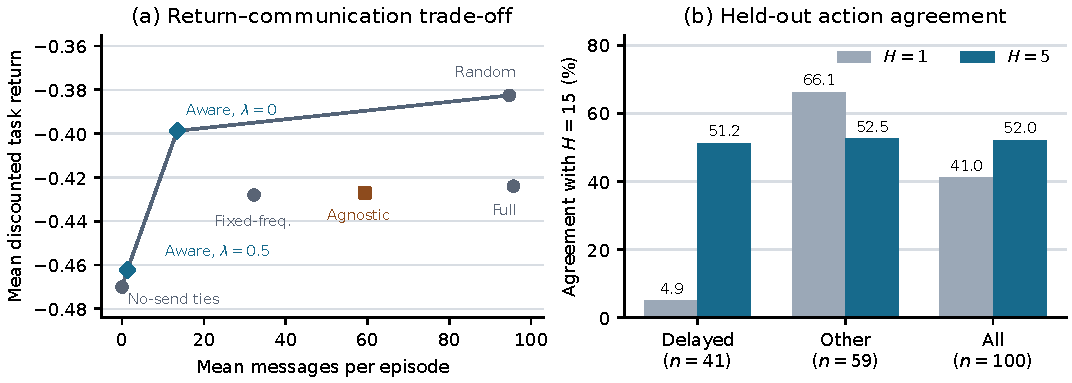
\includegraphics[width=\linewidth]{figures/findings.pdf}
 \caption{Unrestricted discounted return versus messages and oracle agreement by horizon. The episode comparison uses ten seeds per condition. Delayed agreement uses 41 held-out contexts, with the remaining 59 contexts shown separately. The Pareto frontier uses the observed condition means.}
 \label{fig:findings}
\end{figure}

\subsection{Communication, returns and rescues}

The condition table reports discounted return, send volume, and rescues together. At zero cost, aware five-step valuation sent 135 messages in ten episodes, compared with 957 for Full and 594 for Agnostic. Its mean discounted return was $-0.399$, compared with $-0.424$ for Full. The paired interval for Aware minus Full, $[0.005,0.052]$, lies inside the equivalence margin. H2's traffic criterion is therefore met. With the prospectively assigned two-message budget, both valuation policies sent exactly 20 messages across ten episodes. The paired difference in return was $+0.0206$ with interval $[0.0000,0.0603]$, which fails the second H2 criterion. The two policies chose different send times on one seed under the state-dependent eligibility rule.

The rescue outcomes change the practical interpretation. At zero cost Aware evacuated 10 victims and Full evacuated 17. The paired difference was $-0.70$ rescues per episode ($95\%$ CI $[-1.40,-0.10]$). Fixed-frequency evacuated 20 with 323 sends. In the assigned two-message arm, Aware evacuated seven and Agnostic five, yielding $+0.20$ rescues per episode ($95\%$ CI $[0.00,0.50]$). Figure~\ref{fig:findings} uses discounted return for its communication frontier. It is possible to lie on that frontier and still evacuate fewer victims.

\subsection{Receiver differentiation and horizon agreement}

H1's same-report comparison exceeded $0.5$ in 3 of 89 eligible contexts, a fraction of $3.37\%$ ($95\%$ CI $[0,6.74]\%$). Two of the three reports concerned victims. Eleven of the 100 stored contexts had no eligible non-intention report. An exploratory search across every non-intention report finds at least one threshold-exceeding report in 39 of the same 89 contexts. That statistic allows more chances to qualify in contexts with more candidates. The primary H1 test evaluates only the designated report, so its 30\% target remains unmet.

Among 41 delayed contexts, one-step valuation matched the 15-step oracle in 2 and five-step valuation in 21. The paired difference was $19/41=0.4634$, with seed-bootstrap interval $[0.2857,0.6563]$. H3 passes. Across the other 59 contexts agreement decreases from $39/59$ to $31/59$ when the horizon increases. The all-context gain is 11 percentage points. The delayed subset explains the difference between aggregate performance and the specific multi-step decision effect (Figure~\ref{fig:findings}).

\subsection{Cost sensitivity and estimator diagnostics}

The mean seed rate of positive-value sends drops from $13.74\%$ to $1.40\%$ when $\lambda$ rises from 0 to 0.5. The pooled counts are 135 sends in 966 opportunities and 13 in 967, respectively. The H4 estimate uses the mean of seed rates and gives a relative drop of $89.84\%$ ($95\%$ CI $[80.17,95.84]\%$), above the 15\% target. Total rescues decline from ten to seven as sends become more expensive. Since policies visit potentially different states as cost changes, the observed drop reflects both thresholding and changes in the sequence of opportunities.

On the 100 oracle contexts the mean shortlist error was $0.0913$ reward units and mean pair regret was $0.1707$. Among contexts with an oracle pair above the $0.5$ threshold, mean recall was $77.8\%$ ($n=39$). The selected report's recipient regret averaged $0.0064$ and $34$ of $59$ selected sends had positive oracle marginal value. Low recipient regret on selected reports can coexist with greater pair regret because the selected report or the decision to send can differ from the oracle.

\subsection{Separate exploratory studies}

The E01--E12 series used different environment parameters and no-send context samples. In E04 the mean within-estimator standard error at 32 pairs was $0.03550$ with common random numbers and $0.05675$ with independent branch randomness (20 contexts). This measures Monte Carlo precision conditional on the model. E09's 20 early contexts gave $100\%$ all-context agreement at horizon one and $70\%$ at horizon five, a different sample and estimand from H3. E10 included 40 contexts with report ages from 0 to 12 steps. Enabling the freshness heuristic changed no measured context return in that sample. E12 measured mean end-to-end aware decision time of $0.426$ seconds over 40 contexts and recorded seven failure contexts in which aware valuation trailed at least one comparator. In the exploratory four-discount by six-cost sweep, none of the 24 paired context-return intervals for Aware versus Agnostic excluded zero.

\paragraph{Archived configurations.}
The nested project archive contains separate evaluations under adjacent rescue, discount $0.9$, hazard movement probability $0.3$, and a legacy agnostic score that averages over actual receiver models. Its focused H1 evaluation collected ten eligible contexts per seed and found 156 threshold exceedances in 500 contexts across 50 seeds ($31.2\%$, seed-bootstrap CI $[20.6,42.6]\%$). The interval spans the target. The archive also contains two disjoint blocks of 50 seeds under a whole-horizon five-message quota that used positive values when possible and forced remaining sends at the deadline. All 100 pairs spent the quota. The pooled within-seed Aware-minus-Agnostic return difference was $+0.511$ (CI $[0.289,0.771]$). A separate 50-seed forced-spacing run with the same nominal quota gave $-0.379$ (CI $[-0.791,-0.017]$). These schedules and seed blocks differ, so they provide separate exploratory contrasts. In the archive's four-cost study, rates at costs 0 and 0.5 were $15.16\%$ and $2.87\%$ across 50 paired seeds, a drop of $81.05\%$ (CI $[74.75,85.66]\%$). These runs broaden the evidence across configurations. The current two-message transport experiment remains the basis for the primary verdicts.

\section{Discussion}

Five-step rollouts are most useful in the primary run precisely where the one-step oracle and longer oracle disagree about at least one opportunity. This supports the mechanism that communication can change the sequence of actions before it changes reward. The result is conditional on an oracle-defined subset and the simulator's fixed policies. The five-step selector still matches the delayed reference only about half the time. A useful practical study would test a sender-local trigger for when to spend computation on a longer horizon.

The actionable budget makes the receiver comparison more informative. The former fixed-step arm sent 29 intention reports across 40 sends and the two methods never differed in episode return. The new arm spent all 40 sends on victim or hazard reports and produced a positive return difference on three paired seeds. The interval still includes zero, and the rescues also vary across the same small set of seeds. A better average in this rerun is compatible with no repeatable advantage at the assigned quota.

The gap between rescues and discounted return matters for this task. A unit of reward at step 20 carries weight $0.8^{20}\approx 0.0115$. Early progress and later evacuations can therefore move the two metrics in different directions. H2's return-based traffic criterion should be read as a claim about the defined objective. Rescue count provides a complementary operational endpoint. Both outcomes should remain visible when considering changes to the discount or message policy.

\section{Limitations and future work}

Only one Scout sends in the primary design. The policies are fixed heuristics, the hazard and observation models are simplified, and the software charge does not model bandwidth, latency, or contention. The particle filter approximates the recipient's memory from what the sender knows it delivered. The estimated posterior and finite-sample oracle both have error, and truncated rollouts omit effects after their evaluation horizon. The greedy maximization can favor noisy estimates or leave out useful pairs after shortlisting. Future experiments can vary the shortlist and Monte Carlo budgets jointly and evaluate more independent layouts with action-relevant opportunities. A larger independent seed block, reserved before tuning, would sharpen the equal-budget estimate and the rescue comparison.

\section{Contributions}

The statuses below describe the assigned deliverables recorded in the proposal and the final workspace. Individual authorship of specific files and runs remains unable to verify from the available history.

\paragraph{Chitiveli Hemcharan Varma --- Fulfilled.} The SAR-Grid simulator, role-specific actions, victim transport, hazard transitions, local observations, communication timing and validation tests are present. The test suite guards the actual simulator during online selector calls.
\paragraph{Guransh Kaur Saran --- Fulfilled for the assigned core.} The three fixed task policies, Never, Random, Full and Fixed-frequency baselines, and matched-seed runner are present. The optional learned-baseline integration was not fulfilled.
\paragraph{Kowel P Laloo --- Fulfilled.} The 64-particle receiver model, paired estimator, receiver-aware and agnostic selection, candidate filter, freshness feature, and offline oracle comparisons are present and exercised in the results.
\paragraph{Omm Arindam --- Fulfilled.} The H1--H4 protocols, metric and seed-level analyses, budget/cost/horizon experiments, runtime and failure studies, result traces, and report integration are present.

\section{Conclusion}

In this simulator, five-step valuation improved delayed-case oracle agreement and increasing the cost strongly reduced sending. The designated report rarely showed the prespecified receiver gap, and the actionable equal-budget test did not establish an aware return advantage. Receiver-aware valuation reduced traffic relative to Full under the discounted-return criterion while evacuating fewer victims. Together these outcomes identify where downstream simulation helps and where the communication policy still needs stronger evidence.

\bibliographystyle{unsrt}
\bibliography{references}
\end{document}
